\documentclass[12pt]{article}
\author{Alex Ho}
\title{FYS4150 - Computational Physics \\ Project 4}
\usepackage{listings}
\usepackage{graphicx}
\usepackage{verbatim}
\usepackage{amsmath}
\usepackage{float}
\usepackage[utf8]{inputenc}
\usepackage{xcolor}
\usepackage{booktabs}
\usepackage{hyperref}
\usepackage{placeins}


\lstset{
language=Python,
basicstyle=\ttfamily,
otherkeywords={self},             
keywordstyle=\ttfamily\color{blue!90!black},
keywords=[2]{True,False},
keywordstyle={[2]\ttfamily\color{blue!90!black}},
emph={MyClass,__init__},          
emphstyle=\ttfamily\color{red!80!black},    
stringstyle=\color{blue!90!black},
showstringspaces=false,
commentstyle=\color{blue!90!black},
breaklines=true,
tabsize=3,
moredelim=**[is][\color{blue}]{@}{@}
}
\begin{document}
\maketitle
\begin{abstract}

\end{abstract}
\newpage
\tableofcontents
\newpage
\section{Introduction} \label{section:intro}
In fields like thermal dynamics, one will study the phenomena called a \emph{phase transition}. Not only do we study it, but we experience this phenomena on a day-by-day basis. An example of a phase transition is when water turns to steam when we boil the water. More general, a phase transition is when matter changes it's form, either from gas to liquid, or liquid to solid (and vice versa).\\\\
We will in this project use a very popular model, the Ising model, to look at the statistical properties of phase transitions analytically. After that, we will use the Metropolis algorithm to see how well it works with the analytical solution and how our system will be for many spins per dimension.\\\\
All relevant files can be found in this GitHub page:\\\\
\url{https://github.com/AHo94/FYS3150_Projects/tree/master/Project4}

%In fields like thermal dynamics, one will study the phenomena called phase transitions. A phase transition is when matter changes it's form. An example of a phase transition is when water turns into ice, i.e, liquid transitions into solid matter. We will in this project study a very popular model, the Ising model, to simulate phase transitions.

\section{Method} \label{section:methods}
\subsection{The Ising model}
The Ising model is a mathematical model for magnetic systems in statistical mechanics. We will in this project consider phase transitions at finite temperatures. The energy, for a specific microstate $i$, is expressed as
\begin{align}
E_i = -J \displaystyle \sum^N_{< kl >}s_ks_l - \mathcal{B}\sum^N_k s_k
\label{eq:Energy_eq}
\end{align}
With the spins $s_k$ which can take values $s_k = \pm 1$. $N$ is the total number of spins in the system and $J$ is a coupling constant, which we will assume to be $J>0$. The symbol $< kl >$ indicates that we only sum over the nearest neighbouring spin. That is, we only the spin $s_k$ with the closest spin $s_l$. $\mathcal{B}$ is an external magnetic field that is interacting with the magnetic moment between neighbouring spins. For simplicity of this project, we will set $\mathcal{B} = 0$.\\\\
We also have the magnetization (or magnetic moment) defined as
\begin{align}
\mathcal{M} = \displaystyle \sum^N_{j=1} s_j
\label{eq:Magnetization}
\end{align}
What we are interested in is the expectation values of the energy $\langle E \rangle$ and the magnetization $\langle \mathcal{M} \rangle$. In order to do that, we will need a probability distribution
\begin{align}
P_i(\beta) = \frac{e^{-\beta E_i}}{Z}
\label{eq:Probability_dist}
\end{align}
where $\beta = 1/k_bT$, the inverse temperature with $k_b$ as the Boltzmann constant. The partition function $Z$ is given as
\begin{align}
Z = \displaystyle \sum_{i=1}^M e^{-\beta E_i}
\label{eq:Partition_func}
\end{align}
which sums over all possible microstates $M$. With these, we can calculate the expectation value of an arbitrary variable $x$
\begin{align*}
\langle x \rangle = \frac{1}{Z}\sum_i x_i e^{-\beta E_i} \\
\langle x^2 \rangle = \frac{1}{Z}\sum_i x_i^2 e^{-\beta E_i}
\end{align*} 
The variance for this variable is then
\begin{align*}
\sigma_x^2 = \langle x^2 \rangle - \langle x \rangle^2
\end{align*}
We can now use these properties to calculate the heat capacity $C_v$ and susceptibility $\chi$, which are given as
\begin{align*}
C_v &= \frac{\sigma_E^2}{k_BT} \\
\chi &= \frac{\sigma_M^2}{k_BT}
\end{align*}
\subsection{Metropolis algorithm}
In this project, we will use the Monte Carlo algorithm known as the Metropolis algorithm to solve our 2 dimensional lattice numerically. 

The algorithm is as following. For each Monte Carlo cycle we do:
\begin{itemize}
\item \textbf{1)} We start with an arbitrary microstate for the given lattice. We use that microstate to calculate the energy $E_b$
\item \textbf{2)} Choose a random spin in the microstate and flip it (e.g, from $\uparrow$ to $\downarrow$). Now we use that state to calculate the energy $E_t$.
\item \textbf{3)} Calculate the energy difference $\Delta E = E_t - E_b$. 
\item \textbf{4)} If $\Delta E <= 0$, we accept the new spin configuration and use the energy $E_t$. What this means is that the energy has been lowered and we are in a lower state.
\item \textbf{5)} If $ \Delta E > 0$, pick a random number $r$ that is given from a uniform distributor in the range $r \in [0,1]$. Now we have to consider these two cases
\item \textbf{5a)} If $r <= e^{-\beta \Delta E}$, we accept the new spin configuration and use the energy $E_t$.
\item \textbf{5b)} If $ r > e^{-\beta \Delta E}$, we reject this new configuration and flip the chosen spin back to it's original state and use the energy $E_b$.
\item \textbf{6)} Once that is done, we use the given microstate (depending on the cases given above) to calculate the magnetic moment $M_i$.
\item \textbf{7)} Finally, we add the calculated energy and magnetic moment to $E_{sum}$ and $M_{sum}$ respectively. These will the one sample of the Monte Carlo cycle.
\end{itemize}
We repeat this process $N_{mc}$ times (with $N_{mc}$ as the number of Monte Carlo cycles) and multiple samplings which will be summed into $E_{sum}$ and $M_{sum}$. Once that is done, we get the mean energies as
\begin{align*}
\langle E \rangle = \frac{1}{N_{mc}}E_{sum} = \frac{1}{N_{mc}}\displaystyle \sum_i E_i
\end{align*}
With $E_i$ is energy sample of the $i$'th Monte Carlo cycle. Similar expressions are used for the magnetic moment and their squares.
\subsection{Simple 2 $\times$ 2 lattice}
We will first consider a 2$\times$2 lattice, find the analytical expression for partition function $Z$ and find the corresponding expectation value of energy $E$, mean magnetization $|M|$, specific heat $C_V$ and susceptibility $\xi$ as functions of temperature $T$. The boundaries for the lattice will be periodic. We will then compare the Ising model with the analytical expressions later.

For this system, we will assume that every spin has two directions, i.e. our states can be either be in spin up state or spin down state (shorthand notation as $\uparrow$ or $\downarrow$ respectively).

The energy of the Ising model, without an external magnetic field $\mathcal{B}$, is given by
\begin{align*}
E_i = \displaystyle -J \sum_{<kl>}^Ns_k s_l
\end{align*} 
Where $J > 0$ is a coupling constant and $N$ is the total number of spins. The symbol $<kl>$ indicates that we only sum over the neighbours only. The values $s_k = \pm 1$ depends on which state it is in. We let $s_{\downarrow} = -1$ and $s_{\uparrow} = 1$. We also have the magnetic moment is given as
\begin{align*}
M_i = \displaystyle \sum_{<k>}^N s_k
\end{align*}
Since we have a $2\times2=4$ lattice, and we have two spin directions, then the number of microstate (or configuration) is $2^4 = 16$. What this means is that our we can have 16 different energies, as well as 16 different magnetic moment, for each respective microstate. Table \ref{table:All_microstates} shows all the possible microstates.

\begin{table}
\begin{center}
	\begin{tabular}{c c c c}
	Combinations of & ($s_1, s_2, s_3, s_4$)& $s_j = \lbrace \uparrow, \downarrow \rbrace$  = $\lbrace 1, -1 \rbrace$ &\\
	\hline 
	($\uparrow , \uparrow, \uparrow, \uparrow$) & 
	($\uparrow , \uparrow, \uparrow, \downarrow$) & 
	($\uparrow , \uparrow, \downarrow, \uparrow$)  & 
	($\uparrow , \downarrow, \uparrow, \uparrow$) \\
	($\downarrow , \uparrow, \uparrow, \uparrow$)& ($\uparrow, \uparrow, \downarrow, \downarrow$) & ($\uparrow, \downarrow, \uparrow, \downarrow$) & ($\downarrow, \uparrow, \uparrow, \downarrow$) \\
	($\downarrow, \uparrow, \downarrow, \uparrow$)& ($\downarrow, \downarrow, \uparrow, \uparrow$) & ($\uparrow, \downarrow, \downarrow, \uparrow$) & ($\uparrow, \downarrow, \downarrow, \downarrow$) \\
	($\downarrow, \uparrow, \downarrow, \downarrow$) & ($\downarrow, \downarrow, \uparrow, \downarrow$) & ($\downarrow, \downarrow, \downarrow, \uparrow$) & ($\downarrow, \downarrow, \downarrow, \downarrow$) \\
	\hline
	\end{tabular}
\caption{All the microstates possible.}
\label{table:All_microstates}
\end{center}
\end{table}

Figure \ref{fig:Lattice_illustration} shows a $2\times2$ lattice. We see that the point $s_1$ has $s_2$ and $s_3$ as the closest neighbours. Since we are considering periodic boundary conditions, then $s_1$ will connect to $s_2$ and $s_3$ twice. The energy term will then give the term $2(s_1s_2 + s_2s_3)$ for the point $s_1$. It does not include $s_4$ as it is not the closest neighbour to $s_1$. 
\begin{figure}[!h]
\centering
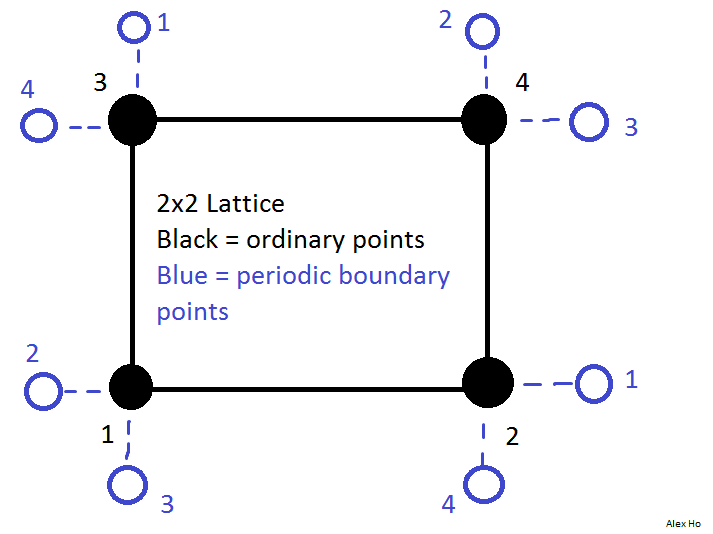
\includegraphics[width=\linewidth]{2x2_lattice_illustration.png}
\caption{An illustration of the $2\times 2$ lattice. The black points corresponds to the ordinary points $s_1, s_2, s_3, s_4$ (as point 1, 2, 3, 4 in the figure respectively). The blue points corresponds periodic boundary points.}
\label{fig:Lattice_illustration}
\end{figure}

We can then continue to add more terms using the three other points, but we need to be careful to not include the connections of the points we previously have considered, which is to prevent double counting. Doing this, the energy for each microstate $i$ will be
\begin{align}
E_i = -2J\displaystyle \sum_{s_1 = \pm1} \sum_{s_2 = \pm1} \sum_{s_3 = \pm1} \sum_{s_4 = \pm1}(s_1s_2 + s_1s_3 + s_2s_4 + s_3s_4)
\label{eq:Energy}
\end{align}
Similarly for the magnetic moment we get when we sum over all microstates 
\begin{align}
M_i = \displaystyle \sum_{s_1 = \pm1} \sum_{s_2 = \pm1} \sum_{s_3 = \pm1} \sum_{s_4 = \pm1} (s_1 + s_2 + s_3 + s_4)
\label{eq:Magnetic_moment}
\end{align}
Let us now determine both the energies and magnetic moments for all microstates. Using table \ref{table:All_microstates}, we can determine equation (\ref{eq:Energy}) and (\ref{eq:Magnetic_moment}) to their respective microstate. Table \ref{table:All_energies} and \ref{table:All_magnetic_moment} shows the energies and magnetic momenta (using the same combinations in table \ref{table:All_microstates}) respectively.

\begin{table}
\begin{center}
	\begin{tabular}{c c c c}
	$E_i =$& & &\\
	\hline
	-8J & 0 & 0 & 0\\
	0 & 8J & 0 & 0\\
	0 & 8J & 0 & 0\\
	0 & 0 & 0 & -8J\\
	\hline
	\end{tabular}
\caption{Energies for each respective microstate.}
\label{table:All_energies}
\end{center}
\end{table}

\begin{table}
\begin{center}
	\begin{tabular}{c c c c}
	$M_i = $& & & \\
	\hline
	4 & 2 & 2 & 2\\
	2 & 0 & 0 & 0\\
	0 & 0 & 0 & -2\\
	-2 & -2 & -2 & -4\\
	\hline
	\end{tabular}
\caption{Magnetic moments for each respective microstate.}
\label{table:All_magnetic_moment}
\end{center}
\end{table}

Now that we have the energies of each microstate, we can find an analytical expression for the partition function $Z$ given in \ref{eq:Partition_func}. Using the energies given in table \ref{table:All_energies}, the partition function becomes
\begin{align*}
Z = 2e^{8\beta J} + 2e^{-8\beta J} + 12 e^0 = 4\cosh(8\beta J) + 12
\end{align*}
With the partition function, we can calculate the expectation value of the energy
\begin{align*}
\langle E\rangle = \frac{1}{Z}\displaystyle \sum_i E_ie^{-\beta E_i}
\end{align*}
Summing over all states $i$, with the given energies in table \ref{table:All_energies}, we get
\begin{align*}
\langle E \rangle &= \frac{1}{Z}\left( 2(8J)e^{-8\beta J} + 2(-8J)e^{8\beta J} + 12\times0\times e^0 \right)\\
&= \frac{-32J \sinh(8\beta J)}{4\cosh(8\beta J) + 12}\\
&= \frac{-8J\sinh(8\beta J)}{\cosh(8\beta J) + 3}
\end{align*}
The expectation of the energy squared is then
\begin{align*}
\langle E^2\rangle &= \frac{1}{Z}\displaystyle \sum_i E_i^2 e^{-\beta E_i} \\
&= \frac{1}{Z} \left(2(8J)^2 e^{-8\beta J} + 2(-8J)^2 e^{8\beta J} + 12 \times (0)^2 e^0 \right) \\
&= \frac{4(8J)^2\cosh(8\beta J)}{4\cosh(8\beta J) + 12} \\
&= \frac{64J^2\cosh(8\beta J)}{\cosh(8\beta J) + 3}
\end{align*}
The standard deviation of the energy then becomes
\begin{align*}
\sigma_E^2 &= \langle E^2\rangle - \langle E \rangle^2 \\
&=\frac{64J^2\cosh(8\beta J)}{\cosh(8\beta J) + 3} - \left( \frac{-8J\sinh(8\beta J)}{\cosh(8\beta J) + 3}\right)^2 \\
&= \frac{64J^2}{\cosh(8\beta J) + 3}\left(\cosh(8\beta J) - \frac{\sinh^2(8\beta J)}{\cosh(8\beta J) + 3} \right) \\
&= \frac{64J^2}{\cosh(8\beta J) + 3}\left(\frac{\cosh^2(8\beta J) + 3\cosh(8\beta J)}{\cosh(8\beta J) + 3} - \frac{\sinh^2(8\beta J)}{\cosh(8\beta J) + 3} \right) \\
&= \frac{64J^2}{\cosh(8\beta J) + 3}\left(\frac{1 + 3\cosh(8\beta J)}{\cosh(8\beta J) + 3} \right)\\
&= \frac{64J^2}{(\cosh(8\beta J) + 3)^2}(4+\cosh(8\beta J))
\end{align*}
Dividing by $k_B T$ gives us the specific heat $C_V$
\begin{align*}
C_V = \frac{1}{k_BT} \left( \langle E^2 \rangle
- \langle E \rangle^2 \right) = \frac{64J^2}{k_B T} \frac{(1+3\cosh(8\beta J))}{(\cosh(8\beta J) + 3)^2}
\end{align*}
We can do similar calculations to obtain the mean magnetization (or the mean absolute value of the magnetic moment), which then gives us
\begin{align*}
\langle |M|\rangle &= \frac{1}{Z} \displaystyle \sum_i |M_i| e^{-\beta E_i} = \frac{2(e^{8\beta J} + 2)}{\cosh(8\beta J) + 3} \\
\langle M^2\rangle &= \frac{1}{Z}\displaystyle \sum_i M_i^2e^{-\beta E_i} = \frac{8(e^{8\beta J} + 1)}{\cosh(8\beta J) + 3}
\end{align*}
Which we can use to calculate the susceptibility $\chi$
\begin{align*}
\chi = \frac{1}{k_B T} \left(\langle M^2 \rangle - \langle |M| \rangle^2\right) = \frac{8}{k_B T} \frac{(e^{8\beta J}+ \cosh(8\beta J) + \frac{3}{2}))}{(\cosh(8\beta J) + 3)^2}
\end{align*} 
We will now proceed with developing the Ising model numerically, using the Metropolis algorithm, and test the model with the analytical expression that we derived above.
\FloatBarrier

\section{Implementation} \label{section:implement}
All programming are done in C++ and data will be saved in a text file. The plotting part will be done in Python.
\section{Results} \label{section:result}
\subsection*{Comparing with analytical solution}

\section{Conclusion} \label{section:conclusion}

\FloatBarrier
\begin{thebibliography}{1}
    \bibitem{cpyhsics} M. Hjorth-Jensen, \emph{Computational Physics}, 2015, 551 pages
\end{thebibliography}
\end{document}